% Senseigigs — DETAILED architecture figure, research-paper style.
% Companion to senseigigs_arch.tex (the simplified 4-stage slide figure).
% Compile: pdflatex -interaction=nonstopmode senseigigs_arch_detailed.tex
%
% Paper-figure conventions: named components, dashed stage groups whose TITLES SIT
% INSIDE the group (a title placed in the gap between groups is always crossed by a
% connector), data-flow arrows with shape labels, a labels/protocol band, and the
% headline numbers in the figure.
%
% Reflects the SHIPPED pipeline after f96b7f0: base LambdaMART + Tier-1 LambdaMART +
% cross-encoder, fused by weighted RRF (0.4/0.4/0.2).
%
% Typesetting note: hyphenation is DISABLED inside nodes and every box uses explicit
% \\ breaks. Without this, narrow boxes silently hyphenate identifiers ("candi-dates",
% "uni-form", "mxbai-embed-") which looks broken in a figure.
\documentclass[border=12pt]{standalone}
\usepackage[T1]{fontenc}
\usepackage{tikz}
\usetikzlibrary{arrows.meta, positioning, fit, backgrounds, calc}
\usepackage{amssymb}

\definecolor{ioC}{HTML}{2B6CB0}
\definecolor{retC}{HTML}{2F855A}
\definecolor{featC}{HTML}{B7791F}
\definecolor{rankC}{HTML}{C05621}
\definecolor{fuseC}{HTML}{6B46C1}
\definecolor{inkC}{HTML}{2D3748}
\definecolor{dataC}{HTML}{4A5568}

\begin{document}
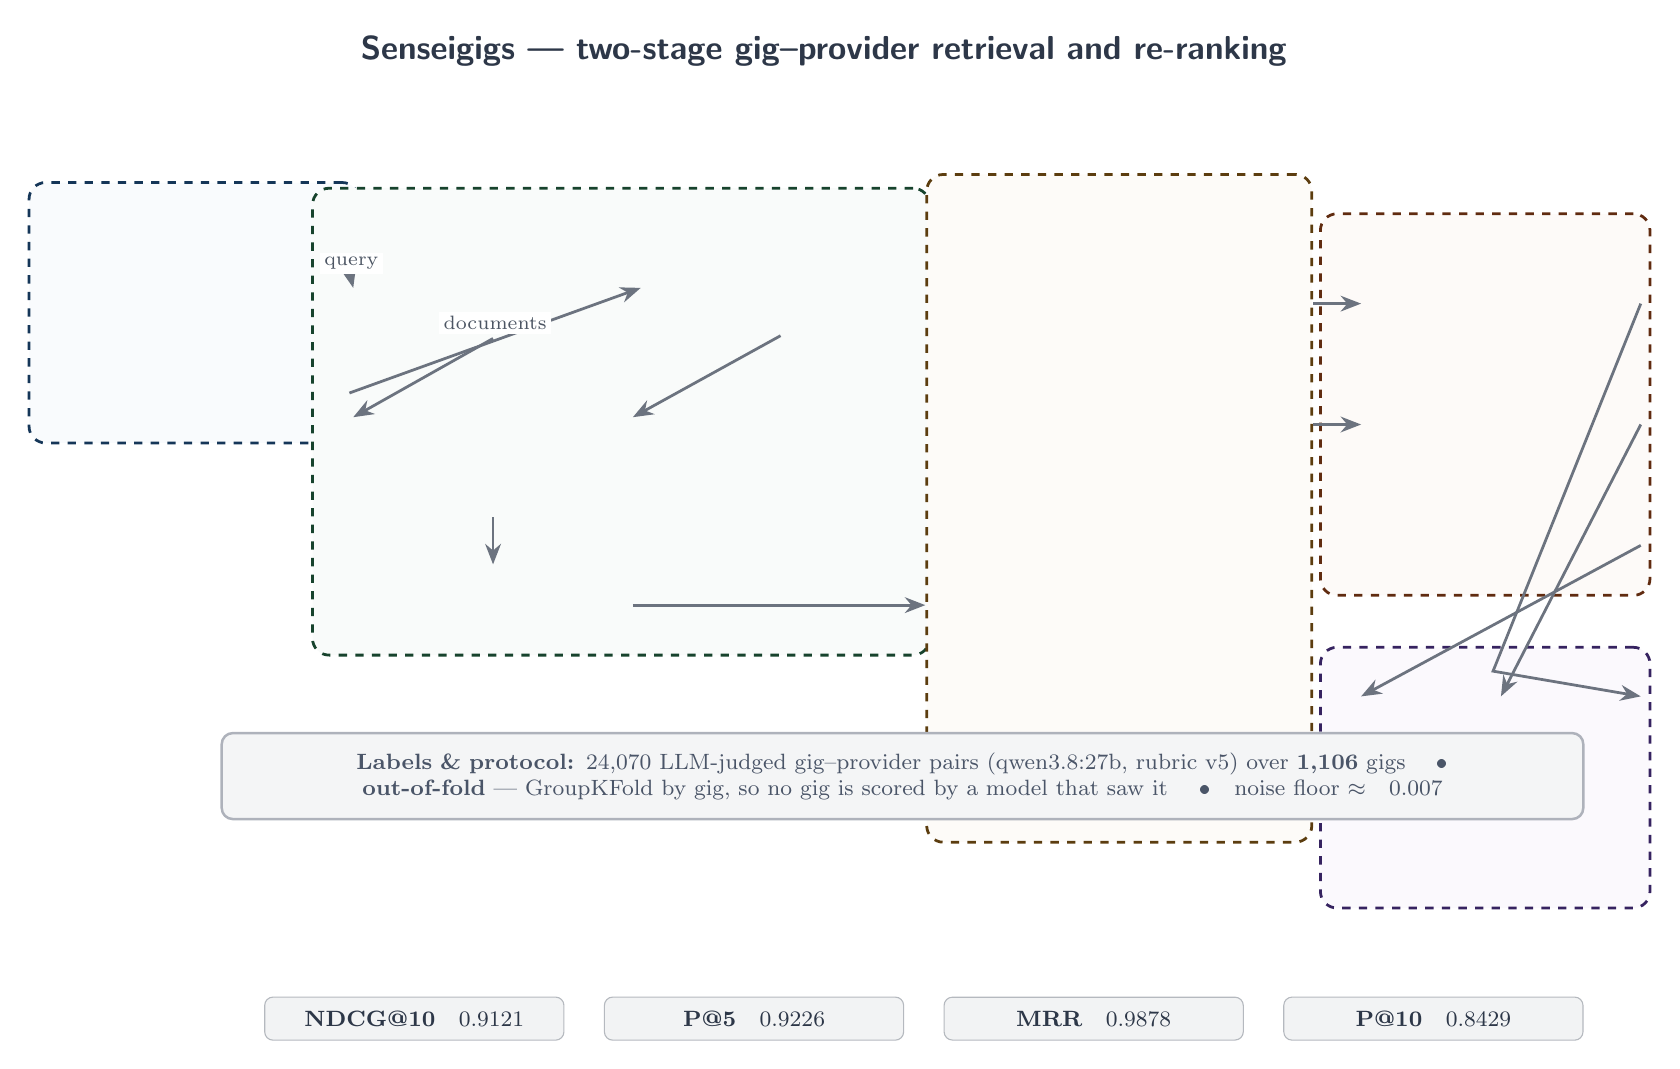
\begin{tikzpicture}[
  font=\sffamily,
  every node/.style={align=center, execute at begin node={\hyphenpenalty=10000\exhyphenpenalty=10000}},
  comp/.style={rounded corners=3pt, draw=#1!80!black, fill=#1!10, line width=1pt,
               inner sep=4.5pt, text width=32mm, minimum height=10mm, font=\footnotesize},
  stitle/.style={font=\small\bfseries, text=#1!55!black},
  stage/.style={rounded corners=6pt, draw=#1!50!black, fill=#1!3, line width=1pt, dashed},
  ar/.style={-{Stealth[length=2.6mm,width=2mm]}, line width=1pt, draw=inkC!70},
  arl/.style={font=\scriptsize, text=inkC!85, fill=white, inner sep=1.6pt},
  tile/.style={rounded corners=3pt, draw=inkC!35, fill=inkC!6, inner sep=5pt,
               font=\footnotesize, text=inkC, minimum width=38mm},
  band/.style={rounded corners=4pt, draw=dataC!45, fill=dataC!6, line width=0.9pt,
               inner sep=7pt, font=\footnotesize, text=dataC, text width=168mm},
]

% ======================= TITLE =======================
\node[font=\sffamily\large\bfseries, text=inkC] (title) at (0,2mm)
  {Senseigigs --- two-stage gig--provider retrieval and re-ranking};

% ======================= INPUTS =======================
\node[comp=ioC] (gig)  at (-78mm,-26mm) {\textbf{Gig posting}\\title $+$ description};
\node[comp=ioC, below=5mm of gig] (prov) {\textbf{Provider profiles}\\\textbf{3{,}024} showcases};
\node[stitle=ioC, anchor=south west, inner sep=3pt] (S0t) at ([xshift=-4mm,yshift=0mm]gig.north west)
  {Inputs};
\node[stage=ioC, fit=(S0t)(gig)(prov)] (S0) {};

% ======================= STAGE 1 =======================
\node[comp=retC] (bm25)  at (-42mm,-28mm) {\textbf{BM25} (Okapi)\\stemmed, title$\times$3,\\synonym expansion};
\node[comp=retC, right=1mm of bm25] (dense) {\textbf{Dense encoder}\\mxbai-embed-large-v1\\1024-d};
\node[comp=retC, below=10mm of bm25] (rrf1) {\textbf{Reciprocal}\\textbf{Rank Fusion}\\$k=60$, uniform};
\node[comp=retC, below=6mm of rrf1] (cand) {\textbf{top-50 candidates}\\per gig};
\node[stitle=retC, anchor=south west, inner sep=3pt] (S1t) at ([xshift=-4mm,yshift=0mm]bm25.north west)
  {Stage 1 --- Retrieval};
\node[stage=retC, fit=(S1t)(bm25)(dense)(rrf1)(cand)] (S1) {};

% ======================= STAGE 2 =======================
\node[comp=featC] (f1) at (36mm,-28mm) {\textbf{Retrieval (6)}\\bm25\_score/rank\\dense\_cosine/rank\\rrf\_score/rank};
\node[comp=featC, below=3mm of f1] (f2) {\textbf{SkillsFuture tags (8)}\\tag\_level, cat\_any,\\spec\_cov, skill\_cov,\\skill\_idf\_cov, skill\_soft};
\node[comp=featC, below=3mm of f2] (f3) {\textbf{Taxonomy graph (6)}\\skill\_sib\_cov,\\skill\_cat\_cov, spec\_cat\_cov,\\graph\_dist\_mean/min};
\node[comp=featC, below=3mm of f3] (f4) {\textbf{Crosses $+$ prior (5)}\\tl\_x\_rank, speccov\_x\_tl,\\skillcov\_x\_tl,\\prov\_prior, prov\_ct};
\node[stitle=featC, anchor=south west, inner sep=3pt] (S2t) at ([xshift=-4mm,yshift=0mm]f1.north west)
  {Stage 2 --- Feature families};
\node[stage=featC, fit=(S2t)(f1)(f2)(f3)(f4)] (S2) {};

% ======================= STAGE 3 =======================
\node[comp=rankC] (r1) at (86mm,-30mm) {\textbf{LambdaMART}\\base --- 17 features};
\node[comp=rankC, below=5mm of r1] (r2) {\textbf{LambdaMART}\\Tier-1 --- 28 features};
\node[comp=rankC, below=5mm of r2] (r3) {\textbf{Cross-encoder}\\fine-tuned MiniLM-L6};
\node[stitle=rankC, anchor=south west, inner sep=3pt] (S3t) at ([xshift=-4mm,yshift=0mm]r1.north west)
  {Stage 3 --- Rankers};
\node[stage=rankC, fit=(S3t)(r1)(r2)(r3)] (S3) {};

% ======================= STAGE 4 (below Stage 3) =======================
\node[comp=fuseC, below=14mm of r3] (fus) {\textbf{Weighted RRF}\\$0.4\,/\,0.4\,/\,0.2$};
\node[comp=fuseC, below=5mm of fus] (out) {\textbf{Top-10 shortlist}\\calibrated 0--100 scores};
\node[stitle=fuseC, anchor=south west, inner sep=3pt] (S4t) at ([xshift=-4mm,yshift=0mm]fus.north west)
  {Stage 4 --- Fusion};
\node[stage=fuseC, fit=(S4t)(fus)(out)] (S4) {};

% ======================= FLOW =======================
\draw[ar] (gig.east)  -- node[arl, midway, above, yshift=0.6mm] {query} (bm25.west);
\draw[ar] (prov.east) -- node[arl, midway, above, yshift=0.6mm] {documents} (dense.west);
\draw[ar] (bm25.south)  -- (rrf1.north west);
\draw[ar] (dense.south) -- (rrf1.north east);
\draw[ar] (rrf1.south) -- (cand.north);
\draw[ar] (cand.east) -- (S2.west |- cand.east);
\draw[ar] (S2.east |- r1.west) -- (r1.west);
\draw[ar] (S2.east |- r2.west) -- (r2.west);
\draw[ar] (r1.east) -- ($(S4.north)!0.5!(fus.north) + (0mm,0mm)$ |- r1.east) -- (fus.north east);
\draw[ar] (r2.east) -- (fus.north);
\draw[ar] (r3.east) -- (fus.north west);
\draw[ar] (fus.south) -- (out.north);

% ======================= LABELS BAND =======================
\node[band] (lab) at (10mm,-90mm)
  {\textbf{Labels \& protocol:} 24{,}070 LLM-judged gig--provider pairs (qwen3.8:27b, rubric v5)
   over \textbf{1{,}106} gigs \quad\textbullet\quad \textbf{out-of-fold} --- GroupKFold by gig,
   so no gig is scored by a model that saw it \quad\textbullet\quad noise floor $\approx 0.007$};

% ======================= RESULT TILES =======================
\node[tile, anchor=north] (t1) at (-52mm,-118mm) {\textbf{NDCG@10}\quad 0.9121};
\node[tile, right=5mm of t1] (t2) {\textbf{P@5}\quad 0.9226};
\node[tile, right=5mm of t2] (t3) {\textbf{MRR}\quad 0.9878};
\node[tile, right=5mm of t3] (t4) {\textbf{P@10}\quad 0.8429};

\end{tikzpicture}
\end{document}
